% Motivation slides 1-4, shared by text/research_questions_slides.tex and text/slides/motivation_slides.tex
\begin{frame}{Motivation\quad Different ways of obtaining soil moisture}
\scriptsize
\centering
\renewcommand{\arraystretch}{1.25}
\begin{tabular}{@{}p{0.14\textwidth} p{0.26\textwidth} p{0.16\textwidth} p{0.34\textwidth}@{}}
\toprule
Source & How SM is obtained & Depth & Main limitation \\
\midrule
\textbf{Microwave}\newline (SMAP, SMOS, ASCAT, S1)
  & invert:\newline $\sigma^0$ or $T_B = f(\mathrm{SM}, \text{roughness}, \text{vegetation})$
  & top $\sim$5\,cm; informs part of the root zone (Feldman et al., 2023)
  & shallow; assumes vegetation and roughness; coarse (9--40\,km) except S1 \\
\addlinespace[7pt]
\textbf{Optical / thermal}\newline (S2, Landsat, MODIS)
  & empirical relations with surface properties: reflectance and indices; LST--vegetation space (e.g. triangle method, TVDI)
  & skin / surface
  & indirect, site-specific calibration; clouds; canopy hides the soil \\
\addlinespace[7pt]
\textbf{Land-surface models}
  & $d\theta/dt = P - ET - Q - D$, with parameters $p$
  & full profile
  & forcing errors, soil and vegetation parameters, process representation (Koster et al., 2009; Seneviratne et al., 2010) \\
\addlinespace[7pt]
\textbf{Reanalysis}\newline (ERA5-Land)
  & LSM driven by reanalysis meteorology
  & full profile
  & model assumptions dominate deep layers with few observational constraints (Li et al., 2021; Miguez-Macho and Fan, 2021) \\
\addlinespace[7pt]
\textbf{In situ} (ISMN)
  & direct probe measurement
  & several depths
  & point scale; sparse, uneven global coverage \\
\addlinespace[7pt]
\textbf{Data-driven}\newline (ML / DL)
  & $\mathrm{SM} = f_\theta(\text{inputs})$, learned from in-situ labels; no ad-hoc process assumptions
  & any depth with labels
  & needs enough, representative sites; generalisation?; hard to interpret? \\
\bottomrule
\end{tabular}
\end{frame}

\begin{frame}{Motivation\quad Multimodal remote sensing}
\begin{columns}[T,onlytextwidth]
\begin{column}{0.56\textwidth}
\centering
\textbf{\footnotesize 1.\ Optical: reflectance spectrum}\\[2pt]
\includegraphics[width=\linewidth,height=0.42\textheight,keepaspectratio]{textbook/sm_signals.pdf}
\scriptsize
\begin{itemize}
\item Dry and wet soil reflect differently: wetting darkens soil in every band, most in the SWIR (B11, B12)
\item Green and water-stressed vegetation reflect differently: stress lowers NIR and raises SWIR
\end{itemize}
\end{column}
\begin{column}{0.41\textwidth}
\centering
\textbf{\footnotesize 2.\ SAR: scattering mechanisms}\\[2pt]
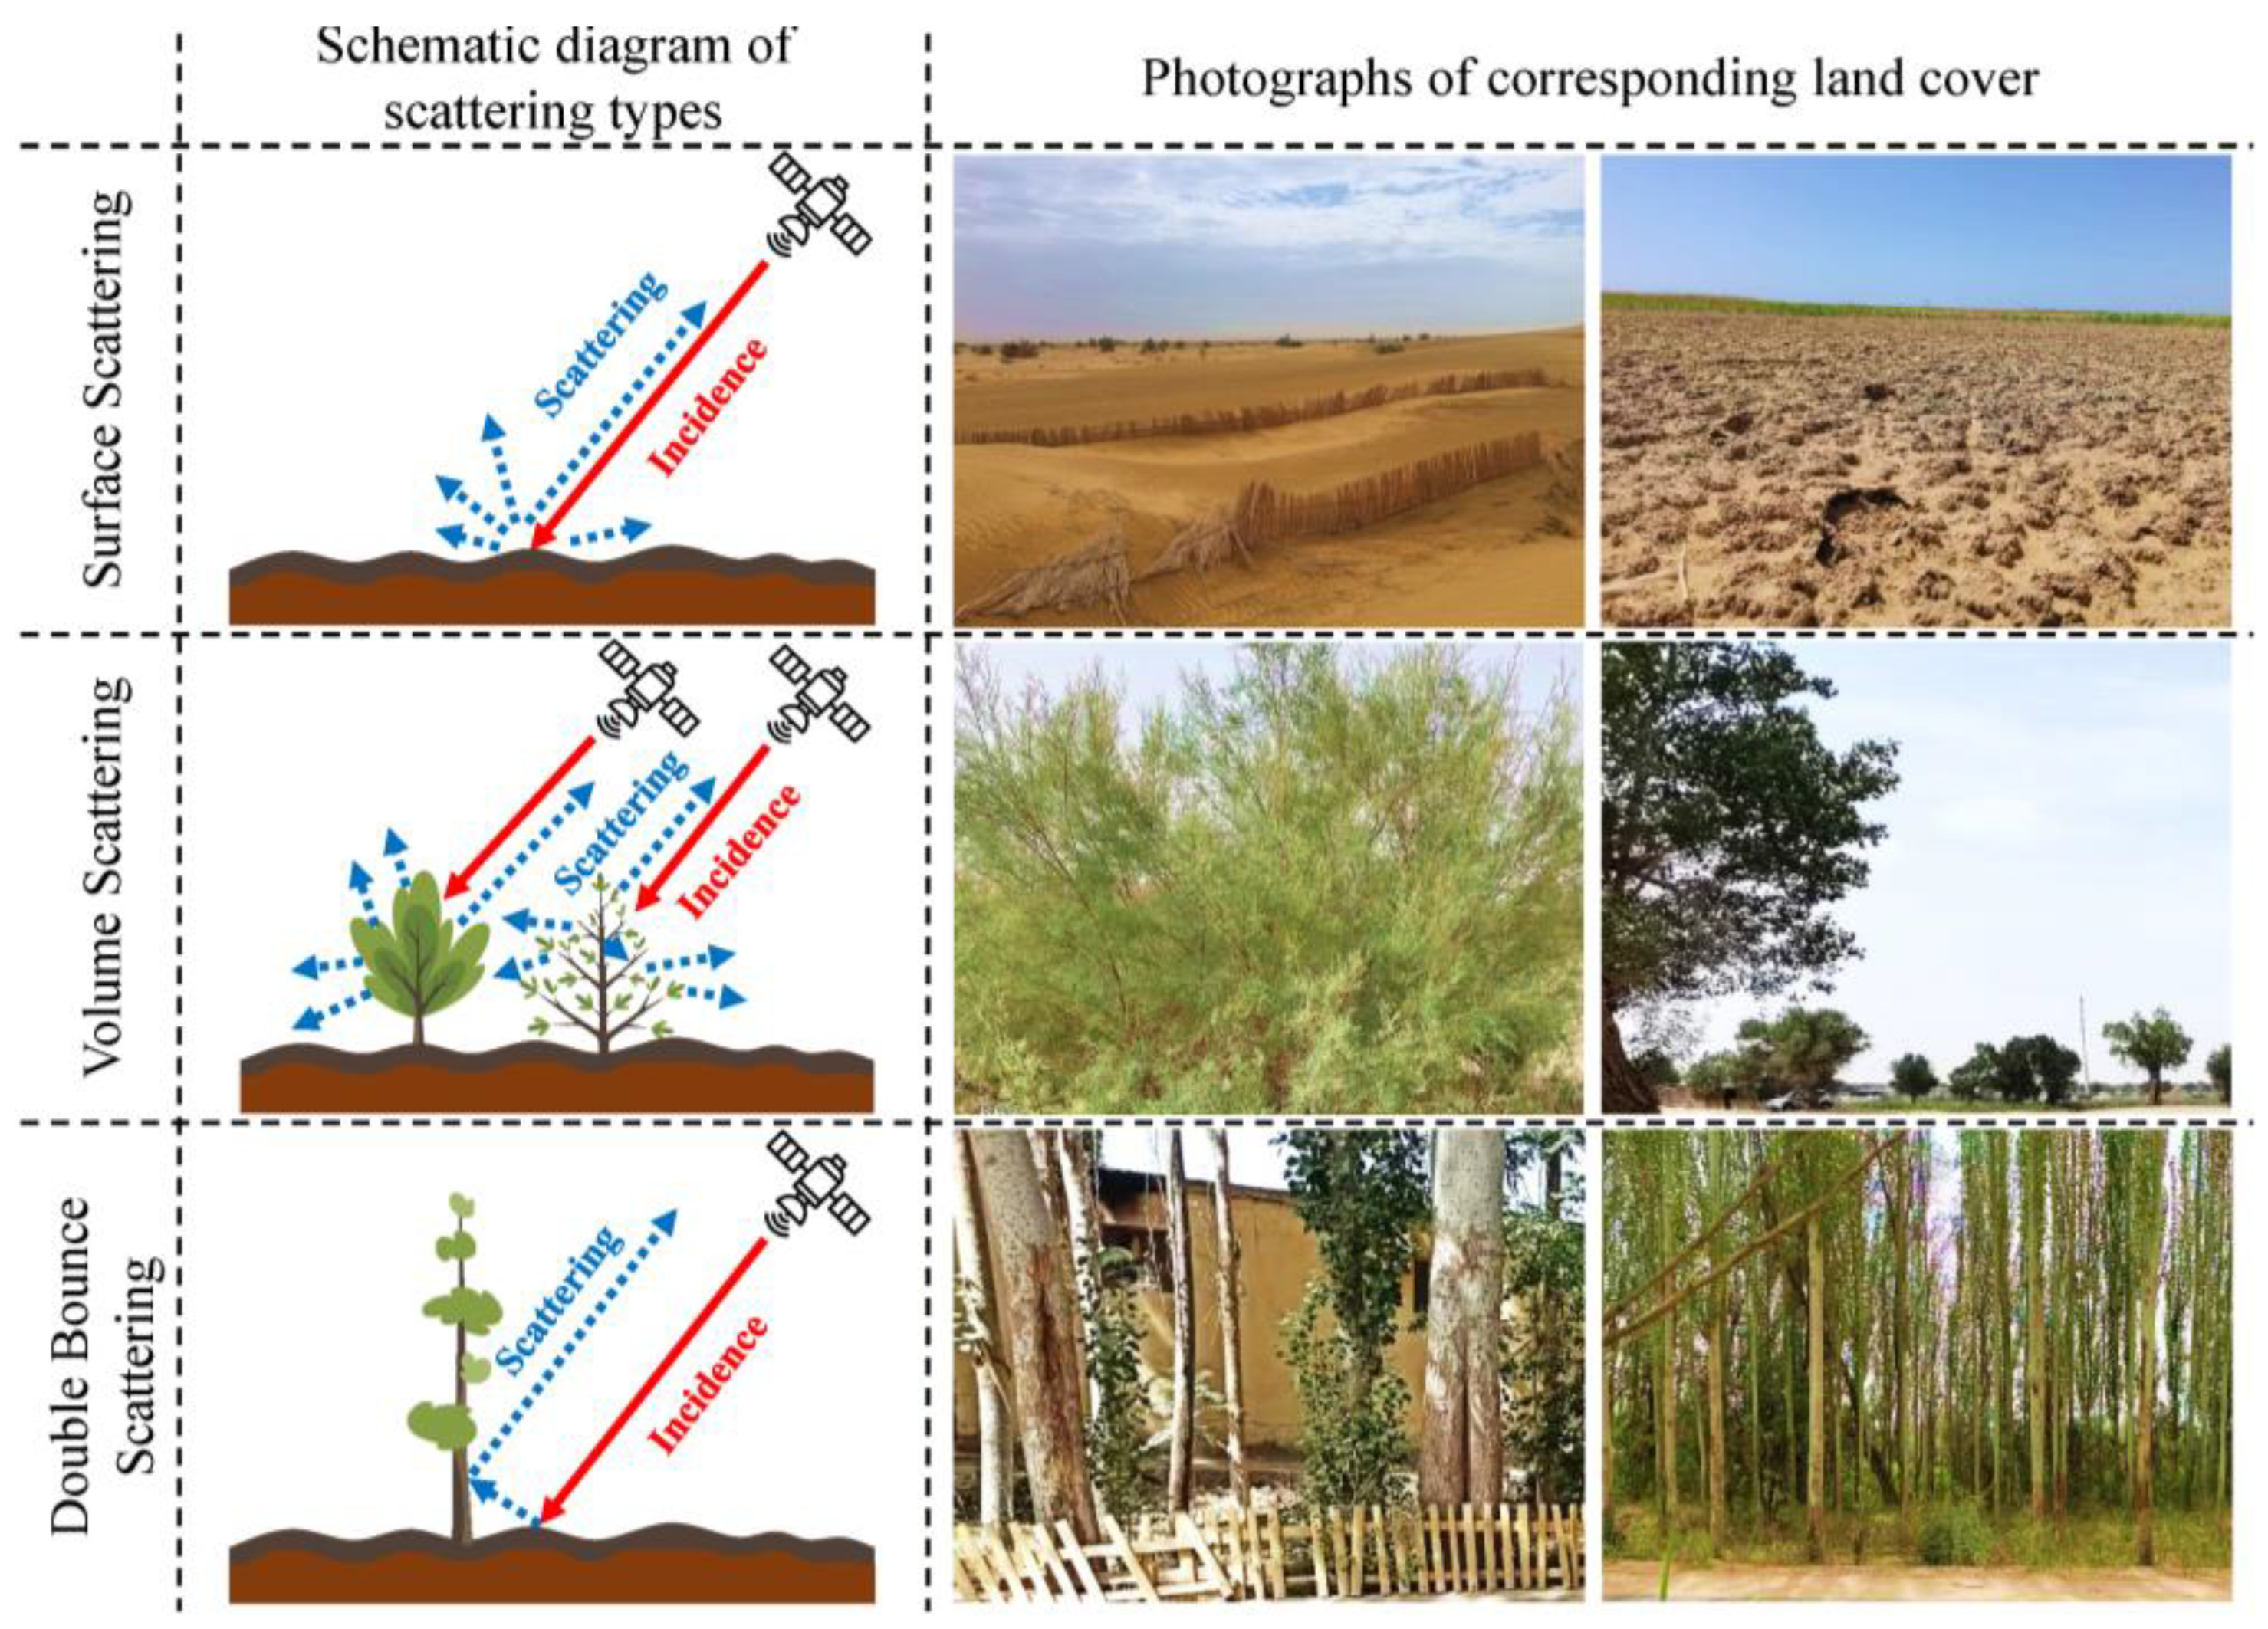
\includegraphics[width=\linewidth,height=0.46\textheight,keepaspectratio]{sensors-25-02512-g003.png}\\[-1pt]
{\tiny Nurmemet et al.\ (2025), \textit{Sensors} 25(8), 2512, doi:10.3390/s25082512}
\scriptsize
\begin{itemize}
\item Bare soil: surface scattering, set by moisture (dielectric) and roughness
\item Canopy: volume and double-bounce scattering mask the soil signal
\end{itemize}
\end{column}
\end{columns}
\end{frame}

\begin{frame}{Motivation\quad Geospatial foundation models (GFMs)}
\centering
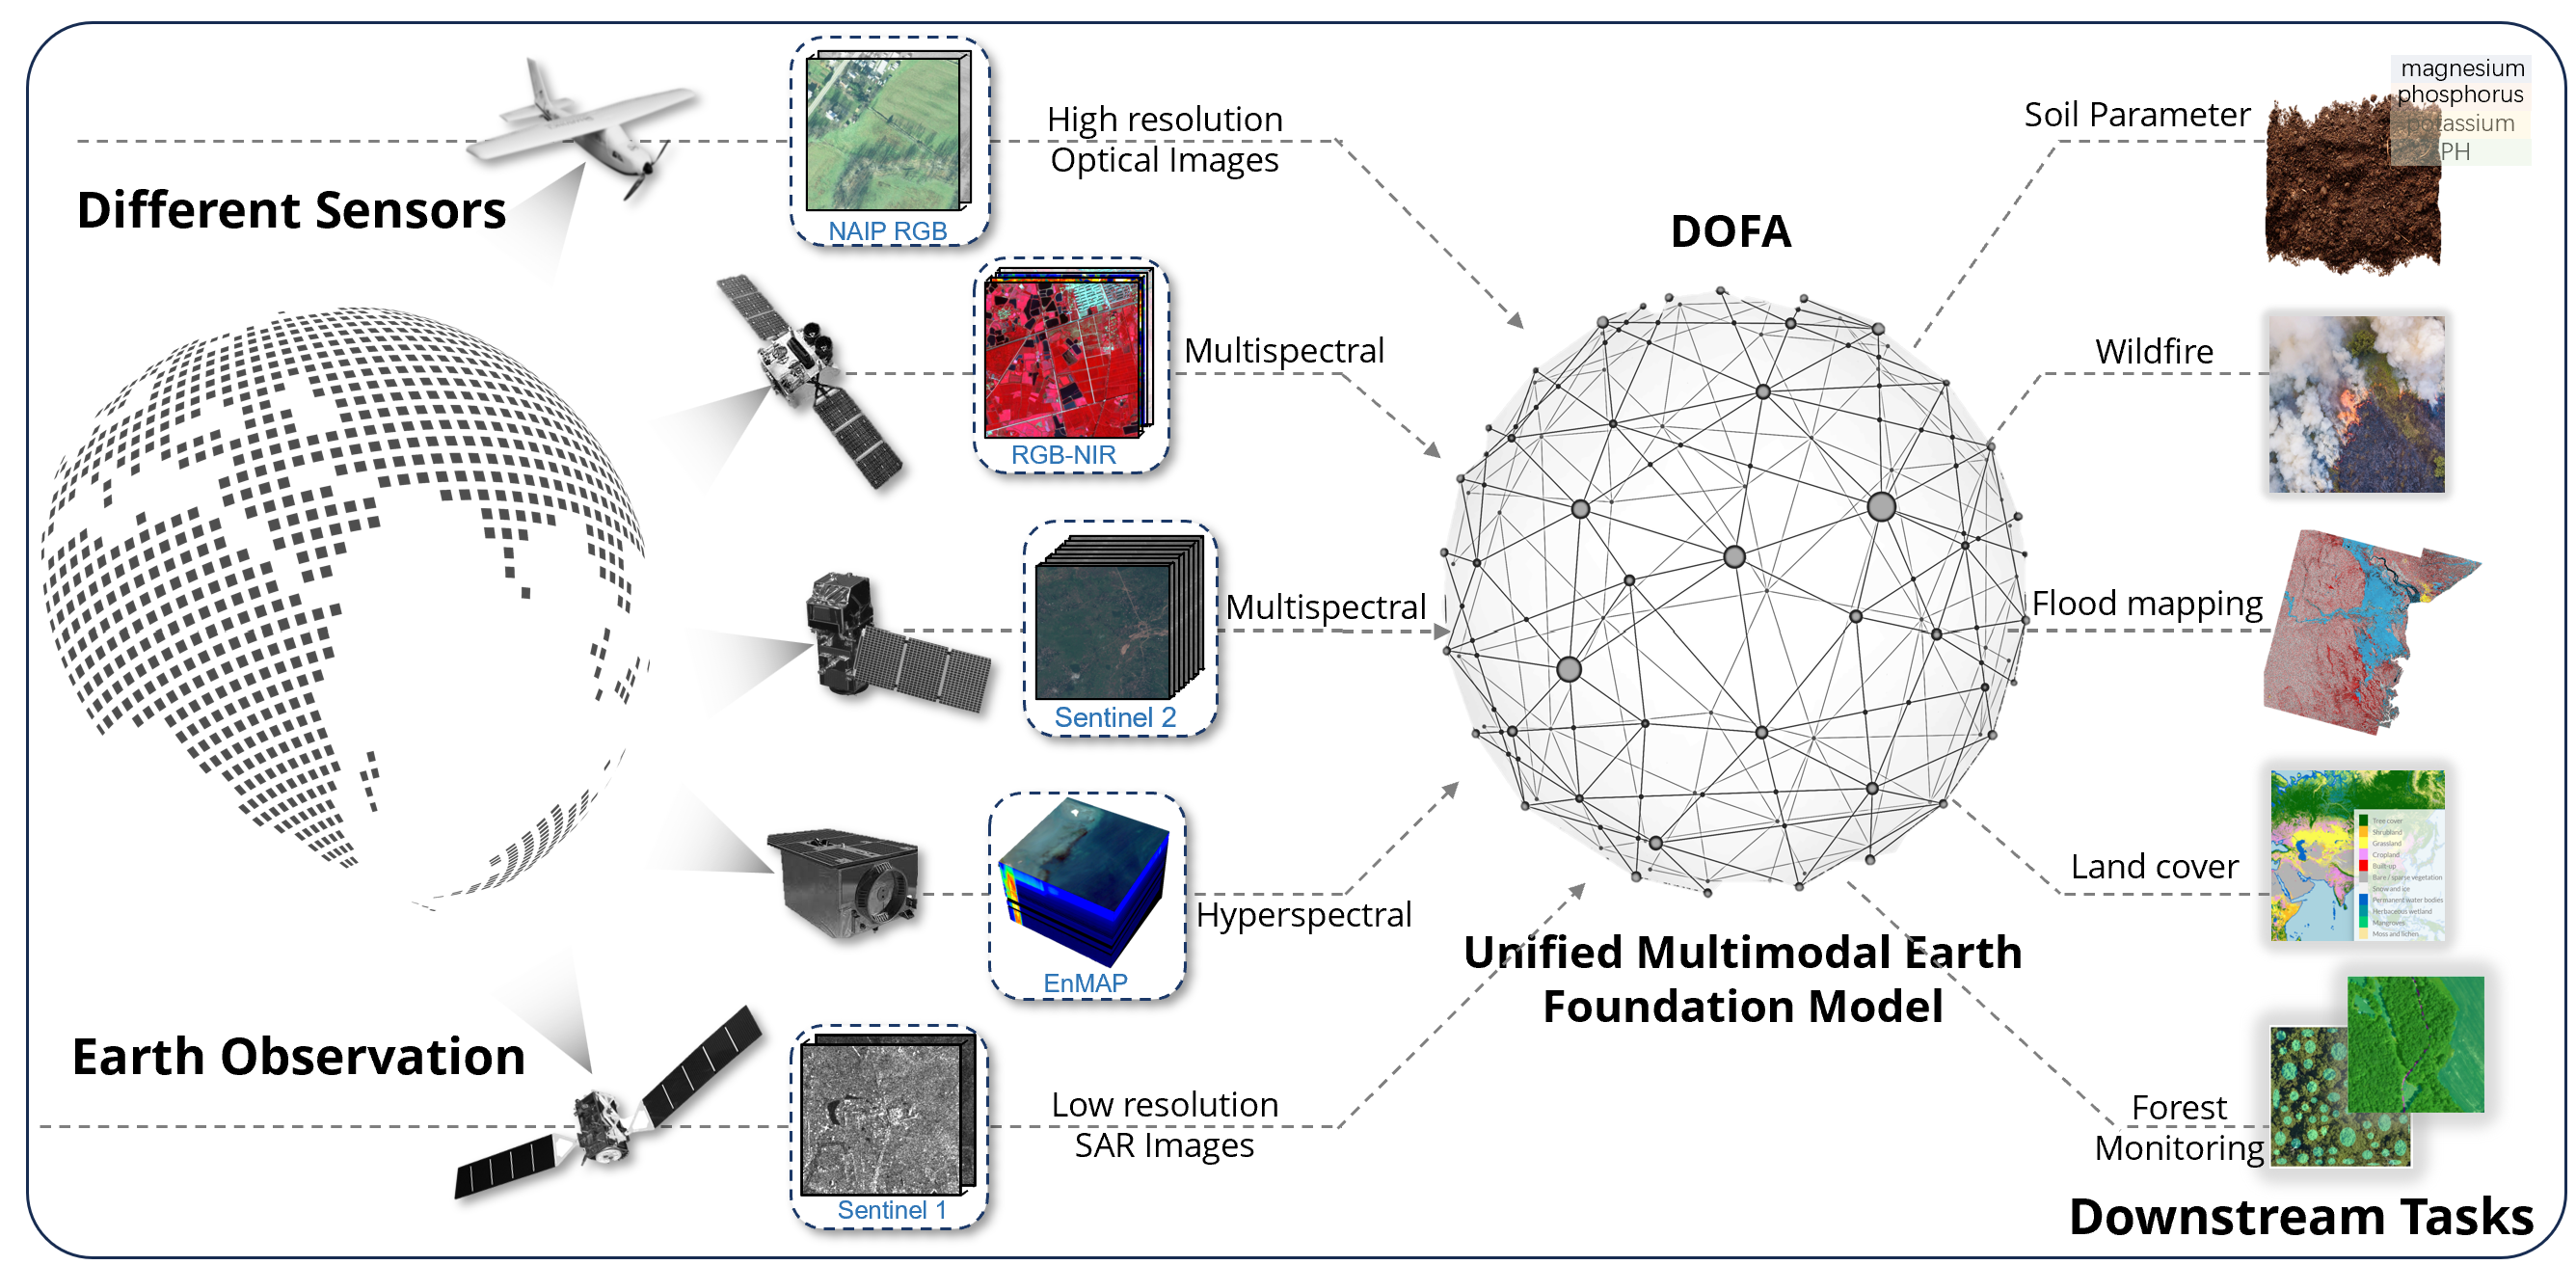
\includegraphics[width=\linewidth,height=0.70\textheight,keepaspectratio]{DOFA1-1.png}\\[-1pt]
{\tiny DOFA: Xiong et al.\ (2024), Neural plasticity-inspired multimodal foundation model for Earth observation, arXiv:2403.15356}\\[6pt]
\begin{beamercolorbox}[wd=0.9\linewidth,center,rounded=true]{block body}
\small\textbf{Once pre-trained on multimodal, unlabelled data, its representation works for many downstream tasks}
\end{beamercolorbox}
\end{frame}

\begin{frame}{Motivation\quad TerraMind embeddings for soil moisture}
\centering
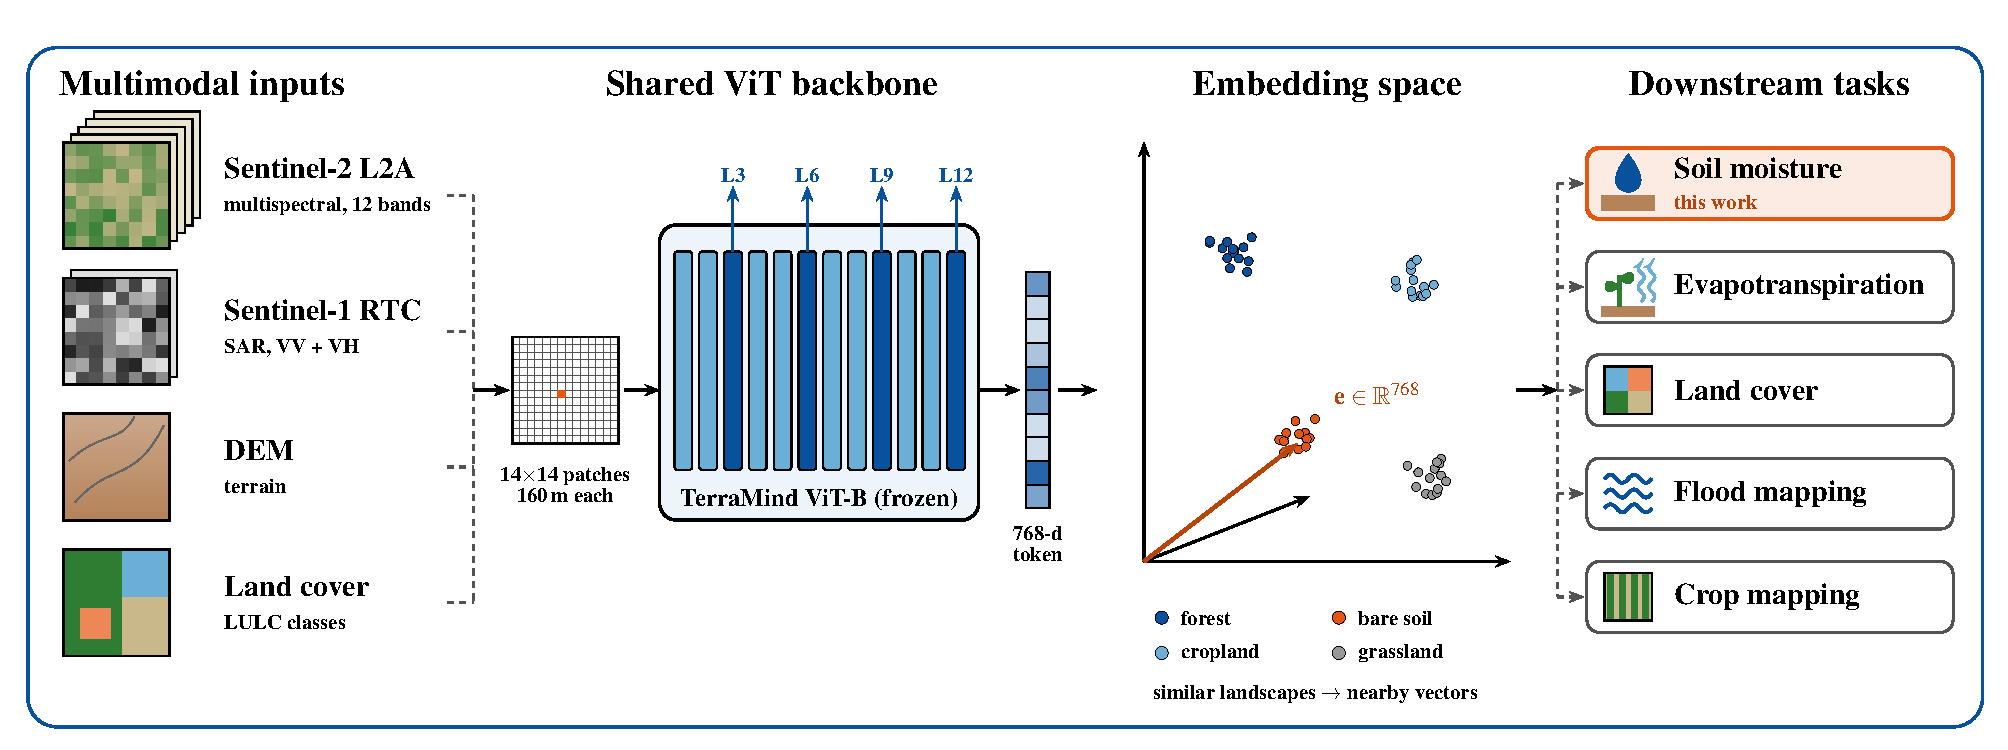
\includegraphics[width=\linewidth,height=0.80\textheight,keepaspectratio]{gfm_embedding_schematic.pdf}\\[4pt]
\footnotesize Frozen TerraMind ViT-B turns each 160\,m patch of S2, S1, DEM and LULC into a 768-d embedding;
the same embedding can serve many tasks; in this case, \textbf{soil moisture}.
\end{frame}
